\section{Optimal Choice}


\subsection{Optimal Bundle}

\slide{Optimal Bundle}{
    We will put together the budget set and the theory of preferences in
    order to examine the optimal choice of consumers.

    The optimal bundle will be the one that lies on the budget line and is
    on the highest indifference curve.

    Well-behaved preferences mean that we can restrict our attention to bundles of goods that lie on the
    budget line and not worry about those beneath the budget line.

    Start at the right-hand corner of the budget line and move to
    the left. As we move along the budget line we note that we are moving to
    higher and higher indifference curves. We stop when we get to the highest
    indifference curve that just touches the budget line.
}


\slide{Optimal Bundle}{
    \begin{center}
        \includegraphics[scale=0.35]{CHOICE1}
    \end{center}
}


\slide{Optimal Bundle}{
    Note an important feature of this optimal bundle: at this choice, the
    indifference curve is tangent to the budget line.

    If the indifference curve weren't tangent, it would cross the budget line, and if it crossed the budget
    line, there would be some nearby point on the budget line that lies above
    the indifference curve.

    Does this tangency condition really have to hold at an optimal choice? Well, it
    doesn't hold in \emph{all} cases. However, what is always true is that at the optimal point, the indifference curve 
    can't cross the budget line.

    When does “not crossing” imply tangent? Let's look at the exceptions.
}


\subsection{Exceptions}

\slide{Exception 1: Kinky Tastes}{
    The indifference curve might have a kink at the optimal choice, and a tangent just isn't defined.
    \begin{center}
        \includegraphics[scale=0.275]{CHOICE2}
    \end{center}
}


\slide{Exception 2: Boundary Optimum}{
    Suppose that the optimal point occurs where the consumption of some good is zero. This represents a
    boundary optimum.
    \begin{center}
        \includegraphics[scale=0.325]{CHOICE3}
    \end{center}
}


\slide{Exception 3: More than One Tangency}{
    Finally, it is possible that there are multiple tangencies.
    \begin{center}
        \includegraphics[scale=0.35]{CHOICE4}
    \end{center}
}


\subsection{Condition for Optimal Bundle}

\slide{Condition for Optimal Bundle}{
    At the optimal bundle, the indifference curve is tangent to the budget line.
    This means that the slope of the indifference curve must be equal to the slope of the budget line.

    \[MRS = \frac{MU_x}{MU_y} = \frac{p_x}{p_y}\]

    Suppose, for example, that the \(MRS = -\frac{1}{2}\) and the price ratio is \(\frac{1}{1}\).
    Economically speaking, this means that the consumer is willing to give up half a unit of good \(y\)
    to get one more unit of good \(x\). Alternatively, the consumer is willing to give up one unit of good
    \(y\) to get two more units of good \(x\). Meanwhile, the market is willing to exchange them on a one-to-one basis.
    
    Thus, the consumer would certainly be willing to give up some of good \(x\) in
    order to purchase a little more of good \(y\).
}



\section{Consumer Demand}


\subsection{Consumer Demand}

\slide{Consumer Demand}{
    The optimal choice of goods 1 and 2 at some set of prices and income is
    called the consumer's demanded bundle.

    A demand function in terms of prices and income is called a \textbf{Marshallian Demand Function}.
    It is denoted as \(x(p_x, p_y, m)\) and \(y(p_x, p_y, m)\).

    A demand function in terms of prices and utility is called a \textbf{Hicksian Demand Function}.
    It is denoted as \(x(p_x, p_y, u)\) and \(y(p_x, p_y, u)\).
}


\subsection{Perfect Substitutes}

\slide{Perfect Substitutes}{
    Suppose we have the general utility function \(U(x,y) = ax + by\) for goods that
    are perfect substitutes. Furthermore, suppose that we have the general budget constraint
    \(p_x x + p_y y = m\).

    To determine the consumer's demand for goods \(x\) and \(y\), we compare the MRS and price ratio.

    \[MRS = \frac{MU_x}{MU_y} = \frac{a}{b}\]
    \[\text{Price ratio} = \frac{p_x}{p_y}\]
}


\slide{Perfect Substitutes}{
    If \(\frac{a}{b} > \frac{p_x}{p_y}\), then the consumer is unwilling to give up \(x\) for \(y\). Why?

    The slope of the budget line is flatter than the slope of the indifference curves, hence the higher indifference curves
    are to the right.

    \begin{center}
    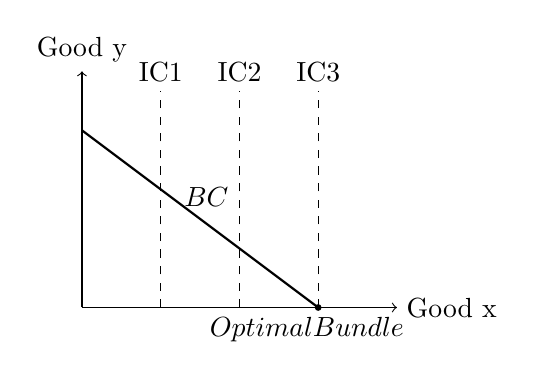
\begin{tikzpicture}[scale=0.5]
    % Axes
    \draw[->] (0,0) -- (8,0) node[right] {Good x};
    \draw[->] (0,0) -- (0,6) node[above] {Good y};

    % Budget line (flatter slope)
    \draw[thick] (0,4.5) -- (6,0) node[above] {};
    \node[below right] at (2.35,3.3) {$\text{BC}$};

    % Indifference curves (vertical lines)
    \draw[dashed] (2,0) -- (2,5.5) node[above] {IC1};
    \draw[dashed] (4,0) -- (4,5.5) node[above] {IC2};
    \draw[dashed] (6,0) -- (6,5.5) node[above] {IC3};

    % Optimal bundle (all x, corner solution)
    \filldraw (6,0) circle (2pt);
    \node[below right] at (3,0) {$\text{Optimal Bundle}$};
    \end{tikzpicture}
    \end{center}

    The demand for good \(x\) is \(x = \frac{m}{p_x}\) and the demand for good \(y\) is \(y = 0\).
}


\slide{Perfect Substitutes}{
    If \(\frac{a}{b} < \frac{p_x}{p_y}\), then the consumer is unwilling to give up \(y\) for \(x\). Why?

    The slope of the budget line is steeper than the slope of the indifference curves, hence the higher indifference curves
    are to the left.

    \begin{center}
    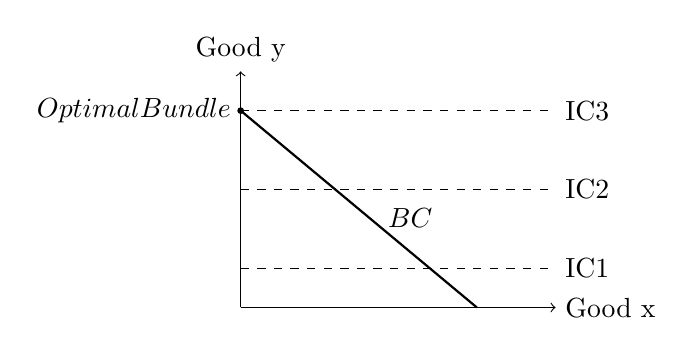
\begin{tikzpicture}[scale=0.5]
    % Axes
    \draw[->] (0,0) -- (8,0) node[right] {Good x};
    \draw[->] (0,0) -- (0,6) node[above] {Good y};

    % Budget line (steeper slope)
    \draw[thick] (0,5) -- (6,0) node[above] {};
    \node[below right] at (3.5,2.75) {$\text{BC}$};

    % Indifference curves (horizontal lines)
    \draw[dashed] (0,1) -- (8,1) node[right] {IC1};
    \draw[dashed] (0,3) -- (8,3) node[right] {IC2};
    \draw[dashed] (0,5) -- (8,5) node[right] {IC3};

    % Optimal bundle (all x, corner solution)
    \filldraw (0,5) circle (2pt);
    \node[left] at (0,5) {$\text{Optimal Bundle}$};
    \end{tikzpicture}
    \end{center}

    The demand for good \(x\) is \(x = 0\) and the demand for good \(y\) is \(y = \frac{m}{p_y}\).
}


\slide{Perfect Substitutes}{
    If \(\frac{a}{b} = \frac{p_x}{p_y}\), then the consumer is indifferent between \(x\) and \(y\). Why?

    The slope of the budget line is equal to the slope of the indifference curves, hence
    there is only one indifference curve and the budget constraint is coincident with it.

    \begin{center}
    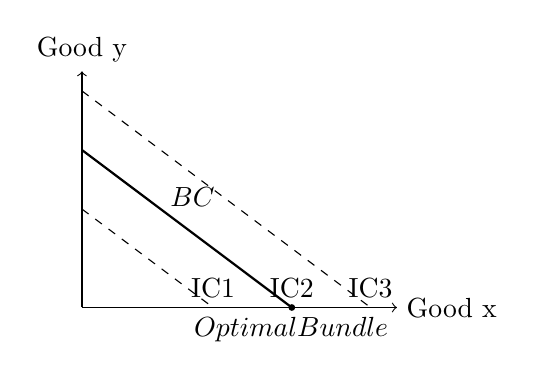
\begin{tikzpicture}[scale=0.5]
    % Axes
    \draw[->] (0,0) -- (8,0) node[right] {Good x};
    \draw[->] (0,0) -- (0,6) node[above] {Good y};

    % Budget line (flatter slope)
    \draw[thick] (0,4) -- (5.33,0) node[above] {};
    \node[below right] at (2,3.3) {$\text{BC}$};

    % Indifference curves (vertical lines)
    \draw[dashed] (0,2.5) -- (3.33,0) node[above] {IC1};
    \draw[dashed] (0,4) -- (5.33,0) node[above] {IC2};
    \draw[dashed] (0, 5.5) -- (7.33,0) node[above] {IC3};

    % Optimal bundle (all x, corner solution)
    \filldraw (5.33,0) circle (2pt);
    \node[below right] at (2.6,0) {$\text{Optimal Bundle}$};
    \end{tikzpicture}
    \end{center}
}


\slide{Perfect Substitutes}{
    Thus, the Marshallian demand function for perfect substitutes is:
    \[(x,y) = 
    \begin{cases}
        \left(\frac{m}{p_x}, 0\right) & \text{if } \ \frac{a}{b} > \frac{p_x}{p_y} \\[0.75em]
        \left(0, \frac{m}{p_y}\right) & \text{if } \ \frac{a}{b} < \frac{p_x}{p_y} \\[0.75em]
        \text{Any point on the budget line} & \text{if } \ \frac{a}{b} = \frac{p_x}{p_y}.
    \end{cases}
    \]
}


\subsection{Perfect Complements}

\slide{Perfect Complements}{
    Suppose we have the general utility function \(U(x,y) = \min\{ax, by\}\) for goods that
    are perfect complements. Furthermore, suppose that we have the general budget constraint
    \(p_x x + p_y y = m\).

    The optimal bundle will be at the corner of the L-shaped indifference curve, where \(ax = by\).
    This implies that \(y = \frac{a}{b}x\).

    Substituting this into the budget constraint gives us:
    \[p_x x + p_y \left(\frac{a}{b}x\right) = m\]
    \[x = \frac{m}{p_x + \frac{a}{b}p_y}\]
    \[y = \frac{a}{b}x = \frac{a}{b} \cdot \frac{m}{p_x + \frac{a}{b}p_y}\]
}


\slide{Perfect Complements}{
    Thus, the Marshallian demand function for perfect complements is:
    \[
    (x,y) = \left(\frac{bm}{bp_x + ap_y}, \frac{am}{bp_x + ap_y}\right)
    \]
}


\subsection{General Strategy}

\slide{General Strategy for Optimal Bundle}{
    \begin{enumerate}
        \item[(1)] Find the MRS by taking the ratio of the marginal utilities \(\left(\frac{MU_x}{MU_y}\right)\)
        \item[(2)] Find the price ratio by taking the ratio of the prices \(\left(\frac{p_x}{p_y}\right)\)
        \item[(3)] Obtain the tangency condition by setting MRS equal to price ratio. This
        will provide a relationship between \(x\) and \(y\).
        \item[(4)] Plug it into the budget constraint to get the demand functions  
    \end{enumerate}
}


\subsection{Cobb-Douglas}

\slide{Consumer Demand for Cobb-Douglas Utility}{
Given the Cobb-Douglas utility function \(U(x,y) = x^{\alpha} y^{\beta}\) and prices \(P_x\) and \(P_y\), we can find the
consumer's demand for goods \(x\) and \(y\).
\[
\quad \frac{\partial U}{\partial x} = \alpha x^{\alpha - 1} y^{\beta}
\quad \text{and} \quad
\frac{\partial U}{\partial y} = \beta x^{\alpha} y^{\beta - 1}.
\]

\[
\text{MRS} = \frac{\frac{\partial U}{\partial x}}{\frac{\partial U}{\partial y}}
= \frac{\alpha x^{\alpha - 1} y^{\beta}}{\beta x^{\alpha} y^{\beta - 1}}
= \frac{\alpha y}{\beta x}.
\]

\[
\text{Price Ratio} = \frac{P_x}{P_y}.
\]
}


\slide{Consumer Demand for Cobb-Douglas Utility}{
\[
\text{Tangency condition} \;\Rightarrow\; \text{MRS} = \text{price ratio}
\]

\[
\frac{\alpha y}{\beta x} = \frac{P_x}{P_y}
\;\Rightarrow\;
P_x = \frac{\alpha y}{\beta x} P_y.
\]

\[
\text{Budget constraint:} \quad P_x x + P_y y = M.
\]

\[
x \left( \frac{\alpha y}{\beta x} P_y \right) + y P_y = M
\;\Rightarrow\;
\frac{\alpha}{\beta} y P_y + y P_y = M.
\]

\[
\Rightarrow\;
y P_y \left( \frac{\alpha}{\beta} + 1 \right) = M
\;\Rightarrow\;
y P_y \left( \frac{\alpha + \beta}{\beta} \right) = M.
\]
}


\slide{Consumer Demand for Cobb-Douglas Utility}{
\[
\Rightarrow\;
y P_y = \left( \frac{\beta}{\alpha + \beta} \right) M
\quad \text{(share of income spent on $y$)}
\]

\[
\Rightarrow\;
y^* = \left( \frac{\beta}{\alpha + \beta} \right) \frac{M}{P_y}
\quad \text{(Marshallian demand)}.
\]
}

\slide{Consumer Demand for Cobb-Douglas Utility}{
Similarly, \(P_y = \frac{\beta x}{\alpha y} P_x.\)

\[
x P_x + y \left( \frac{\beta x}{\alpha y} P_x \right) = M
\;\Rightarrow\;
x P_x + \frac{\beta}{\alpha} x P_x = M.
\]

\[
\Rightarrow\;
x P_x \left( \frac{\beta}{\alpha} + 1 \right) = M
\;\Rightarrow\;
x P_x \left( \frac{\alpha + \beta}{\alpha} \right) = M.
\]

\[
x P_x = \left( \frac{\alpha}{\alpha + \beta} \right) M
\quad \text{(share of income spent on $x$)}
\]

\[
x^* = \left( \frac{\alpha}{\alpha + \beta} \right) \frac{M}{P_x}
\quad \text{(Marshallian demand)}.
\]
}


\slide{Consumer Demand for Cobb-Douglas Utility}{
    Marshallian Demand Functions for Cobb-Douglas Utility:
    \[
    (x^*, y^*) = \left( \frac{\alpha}{\alpha + \beta} \cdot \frac{M}{P_x}, \frac{\beta}{\alpha + \beta} \cdot \frac{M}{P_y} \right).
    \]
}